\documentclass[presentation,aspectratio=43, 10pt]{beamer}
\setbeamersize{text margin left=0.5cm, text margin right=0.5cm}
\usepackage{pifont}
\newcommand{\cmark}{\ding{51}}
\newcommand{\xmark}{\ding{55}}
\usepackage{standalone}

\usepackage{booktabs}
\titlegraphic{\hfill
\includegraphics[height=1.25cm]{durham-logo}}
\usepackage{appendixnumberbeamer}
\usepackage{amsmath}
\usepackage{amssymb}
\usepackage{mathtools}
\usepackage{hyperref}
\usepackage{xspace}
\newcommand{\arxivlink}[2]{{\texttt{arXiv:\,\href{https://arxiv.org/abs/#1}{#1\,[#2]}}}}

\newcommand{\honev}{\ensuremath{{H}^1(\Omega; \mathbb{R}^d)}\xspace}
\newcommand{\ltwov}{\ensuremath{{L}^2(\Omega; \mathbb{R}^d)}\xspace}
\newcommand{\ltwo}{\ensuremath{{L}^2(\Omega)}\xspace}
\newcommand{\inner}[1]{\left\langle #1 \right \rangle}


\usepackage{minted}
\usepackage[url=false,
doi=true,
isbn=false,
style=authoryear,
maxnames=5,
giveninits=true,
uniquename=init,
backend=biber]{biblatex}
\renewcommand{\bibfont}{\fontsize{7}{7}\selectfont}
\addbibresource{references.bib}
\setbeamertemplate{bibliography item}[triangle]
\defbibenvironment{bibliography}
  {\list{}
     {\settowidth{\labelwidth}{\usebeamertemplate{bibliography item}}%
      \setlength{\leftmargin}{\labelwidth}%
      \setlength{\rightmargin}{\labelwidth}%
      \setlength{\labelsep}{\biblabelsep}%
      \addtolength{\leftmargin}{\labelsep}%
      \setlength{\itemsep}{\bibitemsep}%
      \setlength{\parsep}{\bibparsep}}}
  {\endlist}
  {\item}

\setlength{\bibitemsep}{0.5ex}
\setlength{\fboxsep}{1pt}

\renewbibmacro{in:}{}
\DeclareFieldFormat[article]{volume}{\textbf{#1}}
\DeclareFieldFormat{doi}{%
  doi\addcolon%
  {\scriptsize\ifhyperref{\href{http://dx.doi.org/#1}{\nolinkurl{#1}}}
    {\nolinkurl{#1}}}}
\AtEveryBibitem{%
\clearfield{pages}%
\clearfield{issue}%
\clearfield{number}%
}

\DeclareMathOperator{\grad}{grad}
\let\div\relax
\DeclareMathOperator{\div}{div}
\DeclareMathOperator{\curl}{curl}
\DeclareMathOperator{\range}{range}
\DeclareMathOperator{\sym}{sym}
\usetheme{metropolis}
\setbeamertemplate{title graphic}{
  \vbox to 0pt {
    \vspace*{1em}
    \inserttitlegraphic%
  }%
  \nointerlineskip%
}
\metroset{background=light,progressbar=frametitle,numbering=counter,block=fill}

% https://www.dur.ac.uk/marketingandcommunications/marketing/branding/colourpalette/
% Most of these are indistinguishable to those suffering colour blindness
\definecolor{purple}{HTML}{68246D}
\definecolor{blue}{HTML}{002A41}
\definecolor{red}{HTML}{BE1E2D}
\definecolor{cyan}{HTML}{00AEEF}
\definecolor{yellow}{HTML}{FFD53A}
\definecolor{green}{HTML}{00D53A}

\newenvironment{variableblock}[3]
{\setbeamercolor{block body}{#2}
\setbeamercolor{block title}{#3}
\begin{block}{#1}}%
{\end{block}}
  
\newenvironment{challenge}[1]%
{\begin{variableblock}{#1}{bg=red!20,fg=black}{bg=red,fg=white}}%
{\end{variableblock}}

\newenvironment{answer}[1]%
{\begin{variableblock}{#1}{bg=cyan!20,fg=black}{bg=cyan,fg=white}}%
{\end{variableblock}}

\renewenvironment{exampleblock}[1]%
{\begin{variableblock}{#1}{bg=green!20,fg=black}{bg=green,fg=white}}%
{\end{variableblock}}

\setbeamercolor{normal text}{
  fg=blue,
  bg=white
}
\setbeamercolor{alerted text}{
  fg=red
}
\setbeamercolor{example text}{
  fg=blue
}

\setbeamercolor{palette primary}{%
  use=normal text,
  fg=normal text.bg,
  bg=purple,
}

\usetheme{metropolis}

\author{Lawrence Mitchell\inst{1,*} \\
  \and {\scriptsize
    P.~E.~Farrell (Oxford)
    \and
    M.~G.~Knepley (Buffalo)
    \and
    F.~Wechsung (Oxford)}}
\institute{
  \inst{1}Department of Computer Science, Durham University\\
  \inst{*}\texttt{lawrence.mitchell@durham.ac.uk}}

\date{September 27, 2019}
\title{PCPATCH: topological construction of multigrid relaxation methods}

\usepackage{tikz}
\usetikzlibrary{trees,calc,positioning}
\usetikzlibrary{shapes, shapes.geometric,decorations.pathreplacing}
\usetikzlibrary{arrows,arrows.meta,chains,positioning,fit,backgrounds,calc,shapes,
  shadows,scopes,decorations.markings,plotmarks}

\newcommand*{\tettextsize}{\footnotesize}
\tikzstyle{line} = [draw, -, thick]
\tikzstyle{nodraw} = [draw, fill, circle, minimum width=0pt, inner sep=0pt]
\tikzstyle{sieve} = [line, circle, font=\tettextsize, inner sep=0pt,
  minimum size=12pt]

\tikzstyle{cell} = [sieve, fill=blue!60]
\tikzstyle{facet} = [sieve, fill=green!35]
\tikzstyle{edge} = [sieve, fill=red!35]
\tikzstyle{vertex} = [sieve, fill=blue!35]

% https://tex.stackexchange.com/questions/27171/padded-boundary-of-convex-hull
\newcommand{\convexpath}[2]{
  [
  create hullcoords/.code={
    \global\edef\namelist{#1}
    \foreach [count=\counter] \nodename in \namelist {
      \global\edef\numberofnodes{\counter}
      \coordinate (hullcoord\counter) at (\nodename);
    }
    \coordinate (hullcoord0) at (hullcoord\numberofnodes);
    \pgfmathtruncatemacro\lastnumber{\numberofnodes+1}
    \coordinate (hullcoord\lastnumber) at (hullcoord1);
  },
  create hullcoords
  ]
  ($(hullcoord1)!#2!-90:(hullcoord0)$)
  \foreach [
  evaluate=\currentnode as \previousnode using \currentnode-1,
  evaluate=\currentnode as \nextnode using \currentnode+1
  ] \currentnode in {1,...,\numberofnodes} {
    let \p1 = ($(hullcoord\currentnode) - (hullcoord\previousnode)$),
    \n1 = {atan2(\y1,\x1) + 90},
    \p2 = ($(hullcoord\nextnode) - (hullcoord\currentnode)$),
    \n2 = {atan2(\y2,\x2) + 90},
    \n{delta} = {Mod(\n2-\n1,360) - 360}
    in
    {arc [start angle=\n1, delta angle=\n{delta}, radius=#2]}
    -- ($(hullcoord\nextnode)!#2!-90:(hullcoord\currentnode)$)
  }
}

\graphicspath{{./\jobname.figures/}{../pictures/}}

\begin{document}

\maketitle

\begin{abstract}
  Effective relaxation methods are necessary for good multigrid
  convergence. For many equations, standard Jacobi and Gau\ss--Seidel
  are inadequate, and more sophisticated space decompositions are
  required. Examples include problems with semidefinite terms or
  saddle point structure.

  In this talk, I will present PCPATCH, which offers a uniform and
  flexible interface for the topological specification of space
  decompositions for multigrid relaxation methods.

  Implemented in PETSc, and accessed through Firedrake's Python
  preconditioners, PCPATCH facilitates access to a wide range of
  relaxation schemes by simply changing solver options. More complex
  patches can be built by writing a short piece of Python code. I will
  illustrate the utility of this approach with some examples.
\end{abstract}
% \begin{abstract}
%   Small block overlapping, and non-overlapping, Schwarz methods are
%   theoretically highly attractive as multilevel smoothers for a wide
%   variety of problems that are not amenable to point relaxation
%   methods.  Examples include monolithic Vanka smoothers for Stokes,
%   overlapping vertex-patch decompositions for $H(\text{div})$ and
%   $H(\text{curl})$ problems, along with nearly incompressible
%   elasticity, and augmented Lagrangian schemes.

%   While it is possible to manually program these different schemes,
%   their use in general purpose libraries has been held back by a lack
%   of generic, composable interfaces. We present a new approach to the
%   specification and development such additive Schwarz methods in PETSc
%   that cleanly separates the topological space decomposition from the
%   discretisation and assembly of the equations. Our preconditioner is
%   flexible enough to support overlapping and non-overlapping additive
%   Schwarz methods, and can be used to formulate line, and plane
%   smoothers, Vanka iterations, amongst others. I will illustrate these
%   new features with some examples utilising the Firedrake finite
%   element library, in particular how the design of an approriate
%   computational interface enables these schemes to be used as building
%   blocks inside block preconditioners.

%   This is joint work with Patrick Farrell and Florian Wechsung
%   (Oxford), Rob Kirby (Baylor), and Matt Knepley (Buffalo).
% \end{abstract}


\begin{frame}[t]
  \frametitle{Software setting}

  \begin{quote}
    Firedrake (\url{www.firedrakeproject.org}) {\normalfont
      [\ldots]} is an automated system for the solution of
    partial differential equations using the finite element
    method.
  \end{quote}
  \begin{itemize}
  \item Finite element problems specified with \emph{embedded}
    domain specific language, UFL from the
    FEniCS project.
  \item \emph{Runtime} compilation to optimised, low-level (C)
    code.
  \item PETSc for meshes and (algebraic) solvers.\par
    {\hfill \scriptsize \arxivlink{1501.01809}{cs.MS}}

    \nocite{Rathgeber:2016,Alnaes:2014}
  \end{itemize}

  \begin{challenge}{Advert}
    3rd Firedrake user meeting is in Durham 26 \& 27 September 2019.

    {\centering \url{www.firedrakeproject.org/firedrake_19.html}\par}
    
  \end{challenge}
\end{frame}

\begin{frame}[fragile,t]
  \frametitle{UFL makes it easy to write down many complex PDEs}
  \begin{columns}[T]
    \begin{column}{0.47\framewidth}
      \small
      \begin{block}{Rayleigh-B\'enard convection}
        \begin{equation*}
          \begin{split}
            -\Delta u + u\cdot\nabla u + \nabla p +
            \frac{\text{Ra}}{\text{Pr}} \hat{g}T &= 0 \\
            \nabla \cdot u &= 0 \\
            - \frac{1}{\text{Pr}} \Delta T + u\cdot \nabla T &= 0
          \end{split}
        \end{equation*}
        Newton
        \begin{equation*}
          \begin{bmatrix}
            F   & B^T & M_1 \\
            C   & 0   & 0   \\
            M_2 & 0 & K
          \end{bmatrix}
          \begin{bmatrix}
            \delta u \\
            \delta p \\
            \delta T
          \end{bmatrix} =
          \begin{bmatrix}
            f_1 \\
            f_2 \\
            f_3
          \end{bmatrix}
        \end{equation*}
      \end{block}
    \end{column}
    \begin{column}{0.52\framewidth}
\begin{minted}[fontsize=\scriptsize]{python}
from firedrake import *
mesh = ...
V = VectorFunctionSpace(mesh, "CG", 2)
W = FunctionSpace(mesh, "CG", 1)
Z = V * W * W
Ra = Constant(200)
Pr = Constant(6.18)
upT = Function(Z)
u, p, T = split(upT)
v, q, S = TestFunctions(Z)
bcs = ...

F = (inner(grad(u), grad(v))
   + inner(dot(grad(u), u), v)
   - inner(p, div(v))
   + (Ra/Pr)*inner(T*g, v)
   + inner(div(u), q)
   + inner(dot(grad(T), u), S)
   + (1/Pr) * inner(grad(T), grad(S)))*dx

solve(F == 0, upT, bcs=bcs)
\end{minted}
    \end{column}
  \end{columns}
\end{frame}

\begin{frame}[standout]
  What about the solver?
\end{frame}

\begin{frame}[t]
  \frametitle{Some motivating schemes}
  \begin{onlyenv}<1>
    \begin{block}{Coupled multigrid for Stokes/Navier--Stokes}
      \emph{In the SCGS scheme four velocites and one pressure
      corresponding to one finite difference node are simultaneously
      updated by inverting a (small) matrix of equations.}

      \begin{center}
        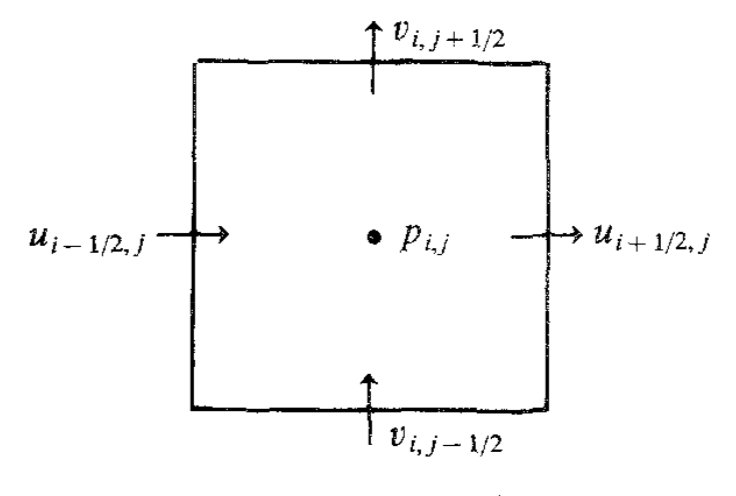
\includegraphics[height=3cm]{vanka}
      \end{center}
      {\hfill \textcite{Vanka:1986}}
    \end{block}
  \end{onlyenv}
  \begin{onlyenv}<2>
    \begin{block}{$p$-independent preconditioners for elliptic problems}
      \emph{[Each subspace is generated from]
      $V_i^p = V^p \cap H^1_0(\Omega_i^{'})$ where $\Omega_i^{'}$ is the open square
      centered at the ith vertex}
      \begin{center}
        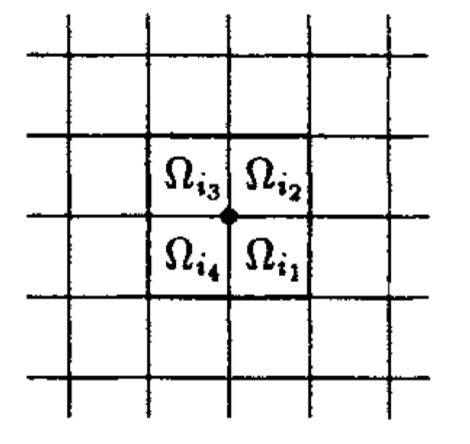
\includegraphics[width=3cm]{pavarino}
      \end{center}
      {\hfill \textcite{Pavarino:1993}}
    \end{block}
  \end{onlyenv}

  \begin{onlyenv}<3>
    \begin{block}{Multigrid for nearly incompressible elasticity}
      \emph{The suggested smoother is a block Jacobi smoother, which takes
      care of the kernel [\dots]. These kernel basis functions are
      captured by subspaces $V_{l,i}$ as shown}
      \begin{center}
        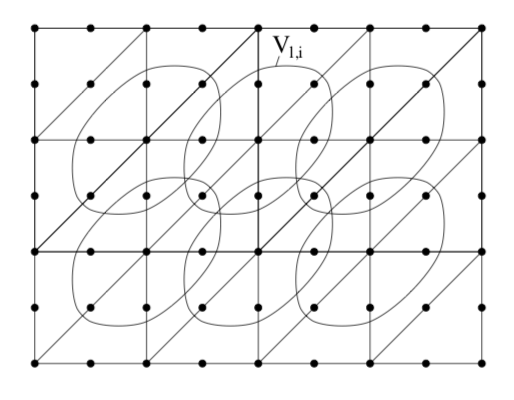
\includegraphics[height=3.25cm]{schoeberl}
      \end{center}
      {\hfill\textcite{Schoeberl:1999}}
    \end{block}
  \end{onlyenv}

  \begin{onlyenv}<4>
    \begin{block}{Multigrid in $H(\div)$ and $H(\curl)$}
      \emph{To define the Schwarz smoothers, we can use a decomposition of
      $V_h$ into local patches consisting of all elements surrounding
      either an edge or a vertex.}

      \begin{center}
        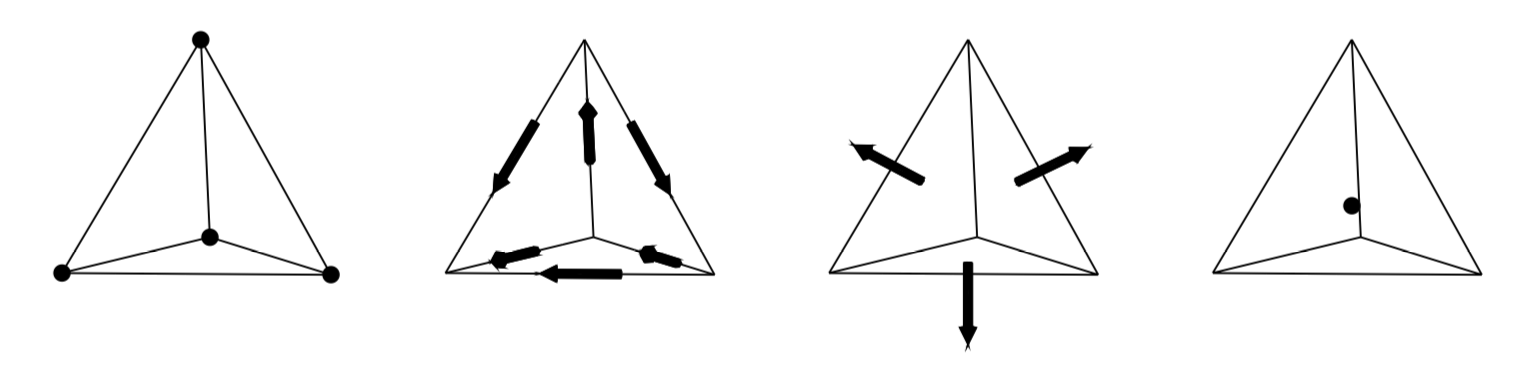
\includegraphics[height=2.5cm]{arnold}
      \end{center}
      {\hfill\textcite{Arnold:2000}}
    \end{block}
  \end{onlyenv}

  \begin{onlyenv}<5>
    \begin{block}{An augmented Lagrangian approach to the Oseen problem}
      \emph{We use a block Gauss-Seidel method [\dots] based on the
      decomposition $V_h = \sum_{i=0}^l V_i$. [\dots For] P2-P0 finite
      elements the natural choice is to gather nodel DOFs for velocity
      inside ovals [around a vertex]}

      \begin{center}
        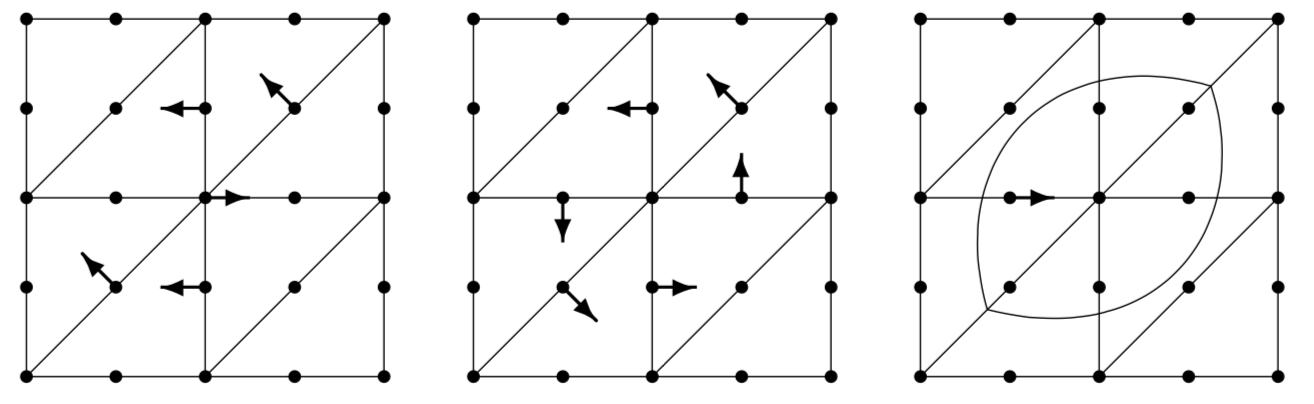
\includegraphics[height=2.5cm]{benzi}
      \end{center}
      {\hfill \textcite{Benzi:2006}}
    \end{block}
  \end{onlyenv}
  \begin{onlyenv}<6>
    \begin{block}{Augmented Lagrangian for 3D Navier--Stokes}
      \begin{center}
        \begin{tikzpicture}[scale=0.55,
          every node/.style={scale=0.55, draw=black, thick, anchor=west},
          grow via three points={one child at (0.0,-0.7) and
            two children at (0.0,-0.7) and (0.0,-1.4)},
          edge from parent path={(\tikzparentnode.210) |- (\tikzchildnode.west)}]
          \node {Continuation}
          child { node {Newton solver with line search}
            child { node {Krylov solver (FGMRES)}
              child { node {Block preconditioner}
                child { node {Approximate Schur complement inverse}}
                child { node {F-cycle on augmented momentum block}
                  child { node {Coarse grid solver}
                    child { node {LU factorization}}
                  }
                  child [missing] {}
                  child { node {Prolongation operator}
                    child { node[fill=red!50, draw=red] {Local solves over coarse cells}}
                  }
                  child [missing] {}
                  child { node {Relaxation}
                    child { node {GMRES}
                      child { node[fill=red!50, draw=red] {Additive star iteration}}
                    }
                  }
                }
              }
            }
          };
        \end{tikzpicture}
      \end{center}
      {\hfill \textcite{Farrell:2018}}
    \end{block}
  \end{onlyenv}
\end{frame}

\begin{frame}
  \frametitle{Unifying observation}
  Smoothers all use block Jacobi/G-S with problem-specific choice of blocks.  
  \begin{itemize}
  \item Decompose space (usually) based on some mesh decomposition
  \item Build and solve little problems on the resulting patches
  \item Combine additively or multiplicatively
  \end{itemize}

  \pause
  \begin{challenge}{Challenge}
    Want to do this inside block preconditioners, and as a multigrid
    smoother.

    Not sufficient to specify dof decomposition on a (single) global matrix.
  \end{challenge}
\end{frame}


\section{\texttt{PCPATCH}}

\begin{frame}[fragile, t]
  \frametitle{\texttt{PCPATCH}}
    \begin{onlyenv}<1-2>
      \begin{challenge}{Requirements}
        \begin{itemize}
        \item Want \emph{flexible} PC $\Rightarrow$ change
          decomposition easily
        \item Need to nest inside more complex solvers
        \end{itemize}
      \end{challenge}
    \end{onlyenv}
    \begin{onlyenv}<2->
      \begin{answer}{Idea}
        \begin{itemize}
        \item Separate topological decomposition from algebraic
          operators
        \item User only provides topological description of patches
        \item Ask discretisation library to make the operators once
          decomposition is obtained
        \end{itemize}
      \end{answer}
    \end{onlyenv}
    \begin{onlyenv}<3->
      \begin{exampleblock}{Library support}
        \begin{itemize}
        \item PETSc (\url{mcs.anl.gov/petsc}): \texttt{DMPlex} + \texttt{PetscDS}\\
          {\scriptsize \verb|-pc_type patch|}
        \item Firedrake (\url{www.firedrakeproject.org}):\\
          {\scriptsize \verb|-pc_type python -pc_python_type firedrake.PatchPC|\\
            \verb|-snes_type python -snes_python_type firedrake.PatchSNES|}
        \end{itemize}
      \end{exampleblock}
    \end{onlyenv}
\end{frame}

\begin{frame}
  \frametitle{Describing patches}
  \begin{itemize}
  \item \texttt{DMPlex} associates dofs with topological entities in mesh
  \item A patch is defined by a set of these entities,
    \texttt{PCPATCH} determines the dofs that correspond to them
  \item Adjacency relations defined using topological queries: often \texttt{star} and \texttt{closure}
  \end{itemize}
  \begin{overlayarea}{\textwidth}{0.6\textheight}
    \begin{uncoverenv}<2->
    \begin{center}
      \begin{tikzpicture}[scale=4]
        \foreach \i/\k in {0/0, 0.5/1, 1/2} {
          \foreach \j/\l in {0/0, 0.5/1, 1/2} {
            \coordinate (v\k\l) at (\i, \j);
          }
        }

        \draw[thick, black, line join=miter] (v00) -- (v10) -- (v20) -- (v21) -- (v22) -- (v12) -- (v02) -- (v01) -- cycle;
        \draw[thick, black, line join=miter] (v01) -- (v11) -- (v21);
        \draw[thick, black, line join=miter] (v10) -- (v11) -- (v12);
        \draw[thick, black, line join=miter] (v01) -- (v10);
        \draw[thick, black, line join=miter] (v02) -- (v11) -- (v20);
        \draw[thick, black, line join=miter] (v12) -- (v21);
        \coordinate (i10) at ($(v10) + (90:0.05)$);
        \coordinate (i20) at ($(v20) + (135:0.07071)$);
        \coordinate (i21) at ($(v21) + (180:0.05)$);
        \coordinate (i12) at ($(v12) + (270:0.05)$);
        \coordinate (i02) at ($(v02) + (315:0.07071)$);
        \coordinate (i01) at ($(v01) + (0:0.05)$);
        \only<2>{\path[fill=purple, opacity=0.5] \convexpath{i01,i02,i12,i21,i20,i10}{0.5pt};}

        \coordinate (o10) at ($(v10) + (90:-0.025)$);
        \coordinate (o20) at ($(v20) + (135:-0.03535)$);
        \coordinate (o21) at ($(v21) + (180:-0.025)$);
        \coordinate (o12) at ($(v12) + (270:-0.025)$);
        \coordinate (o02) at ($(v02) + (315:-0.03535)$);
        \coordinate (o01) at ($(v01) + (0:-0.025)$);
        \phantom{\path[fill=purple, opacity=0.5] \convexpath{o01,o02,o12,o21,o20,o10}{0.5pt};}
        \only<3>{\path[fill=purple, opacity=0.5] \convexpath{o01,o02,o12,o21,o20,o10}{0.5pt};}

        \coordinate (e00) at ($(v00) + (45:0.07071)$);
        \coordinate (e10) at ($(v10) + (135:0.07071)$);
        \coordinate (e11) at ($(v11) + (225:0.07071)$);
        \coordinate (e01) at ($(v01) + (315:0.07071)$);

        \only<4>{\path[fill=purple, opacity=0.5] \convexpath{e00,e01,e11,e10}{0.5pt};}

        \coordinate (ce00) at ($(v00) + (45:-0.03535)$);
        \coordinate (ce10) at ($(v10) + (135:-0.03535)$);
        \coordinate (ce11) at ($(v11) + (225:-0.03535)$);
        \coordinate (ce01) at ($(v01) + (315:-0.03535)$);

        \only<5>{\path[fill=purple, opacity=0.5] \convexpath{ce00,ce01,ce11,ce10}{0.5pt};}

      \end{tikzpicture}

      \only<2>{\texttt{star(vertex)}}
      \only<3>{\texttt{closure(star(vertex))}}
      \only<4>{\texttt{star(edge)}}
      \only<5>{\texttt{closure(star(edge))}}
    \end{center}
    \end{uncoverenv}
  \end{overlayarea}
\end{frame}
\begin{frame}[fragile]
 \frametitle{Describing patches}
 \begin{itemize}
 \item Each patch defined by set of mesh entities
 \end{itemize}
 \begin{block}{Builtin}
   Specify patches by selecting:
   \begin{enumerate}
   \item Mesh entities $\{p_i\}$ to iterate over (e.g.~vertices, cells)
   \item Adjacency relation that gathers points in patch
     \begin{itemize}
     \item[\texttt{star}] entities in $\text{star}(p_i)$
     \item[\texttt{vanka}] entities in $\text{closure}(\text{star}(p_i))$
     \end{itemize}
   \end{enumerate}
 \end{block}
 \begin{block}{User-defined}
   \begin{enumerate}
   \item Custom adjacency relation (e.g. ``only vertices in
     \texttt{closure o star}'')
   \item List of patches, plus iteration order $\Rightarrow$ line-/plane-smoothers
   \end{enumerate}
 \end{block}
\end{frame}

\begin{frame}[fragile]
  \frametitle{Patch assembly}
  \begin{itemize}
  \item If we just want homogeneous Dirichlet, can use list of dofs to
    select from assembled global operator
  \item[\xmark] Doesn't work for other transmission conditions
  \item[\xmark] Doesn't work for nonlinear smoothers
  \item[$\Rightarrow$] Callback interface to get PDE library to
    assemble on each patch
  \end{itemize}
  \begin{block}{Callbacks}
\begin{minted}[fontsize=\scriptsize]{c}
 /* Patch Jacobian */
 UserComputeOp(PC, Vec state, Mat operator, Patch patch, void *userctx);
 /* Patch Residual */
 UserComputeF(PC, Vec state, Vec residual, Patch patch, void *userctx);
\end{minted}
  \end{block}
\end{frame}

\section{Examples}

\begin{frame}
  \frametitle{Which subspace to choose?}

  \begin{itemize}
  \item For symmetric problems, can use kernel decomposition theorem of
    \textcite{Schoeberl:1999} and \textcite{Lee:2007}
  \item Key challenge is to find a decomposition $\{V_i\}$ such that every $u$
    in the kernel $\mathcal{N}$ can be written as $u = \sum_i u_i$
    with $u_i \in V_i \cap \mathcal{N}$.
  \end{itemize}

  \begin{answer}{Characterising the kernel}
    Appropriate discrete de Rham complexes can help us finding the
    support of a basis for $\mathcal{N}$.
  \end{answer}
\end{frame}
\begin{frame}[t,fragile]
  \frametitle{$H(\div)$ multigrid in 2D {\small\parencite{Arnold:1997}}}
  \vspace{-1.5\baselineskip}
  \begin{equation*}
    \text{Find $u \in V \subset H(\div)$ s.t.}\quad (u, v)_{L^2} + \gamma (\div u, \div v)_{L^2} = (f, v)_{L^2} \quad \forall v \in V.
  \end{equation*}
  \vspace*{-\baselineskip}
  \begin{block}{$L^2$ de Rham complex}
    \begin{equation*}
      H^1 \xrightarrow{\grad^\perp}  H(\div) \xrightarrow{\div} L^2
    \end{equation*}
    \vspace*{-2\baselineskip}
    \pause
    \begin{center}
      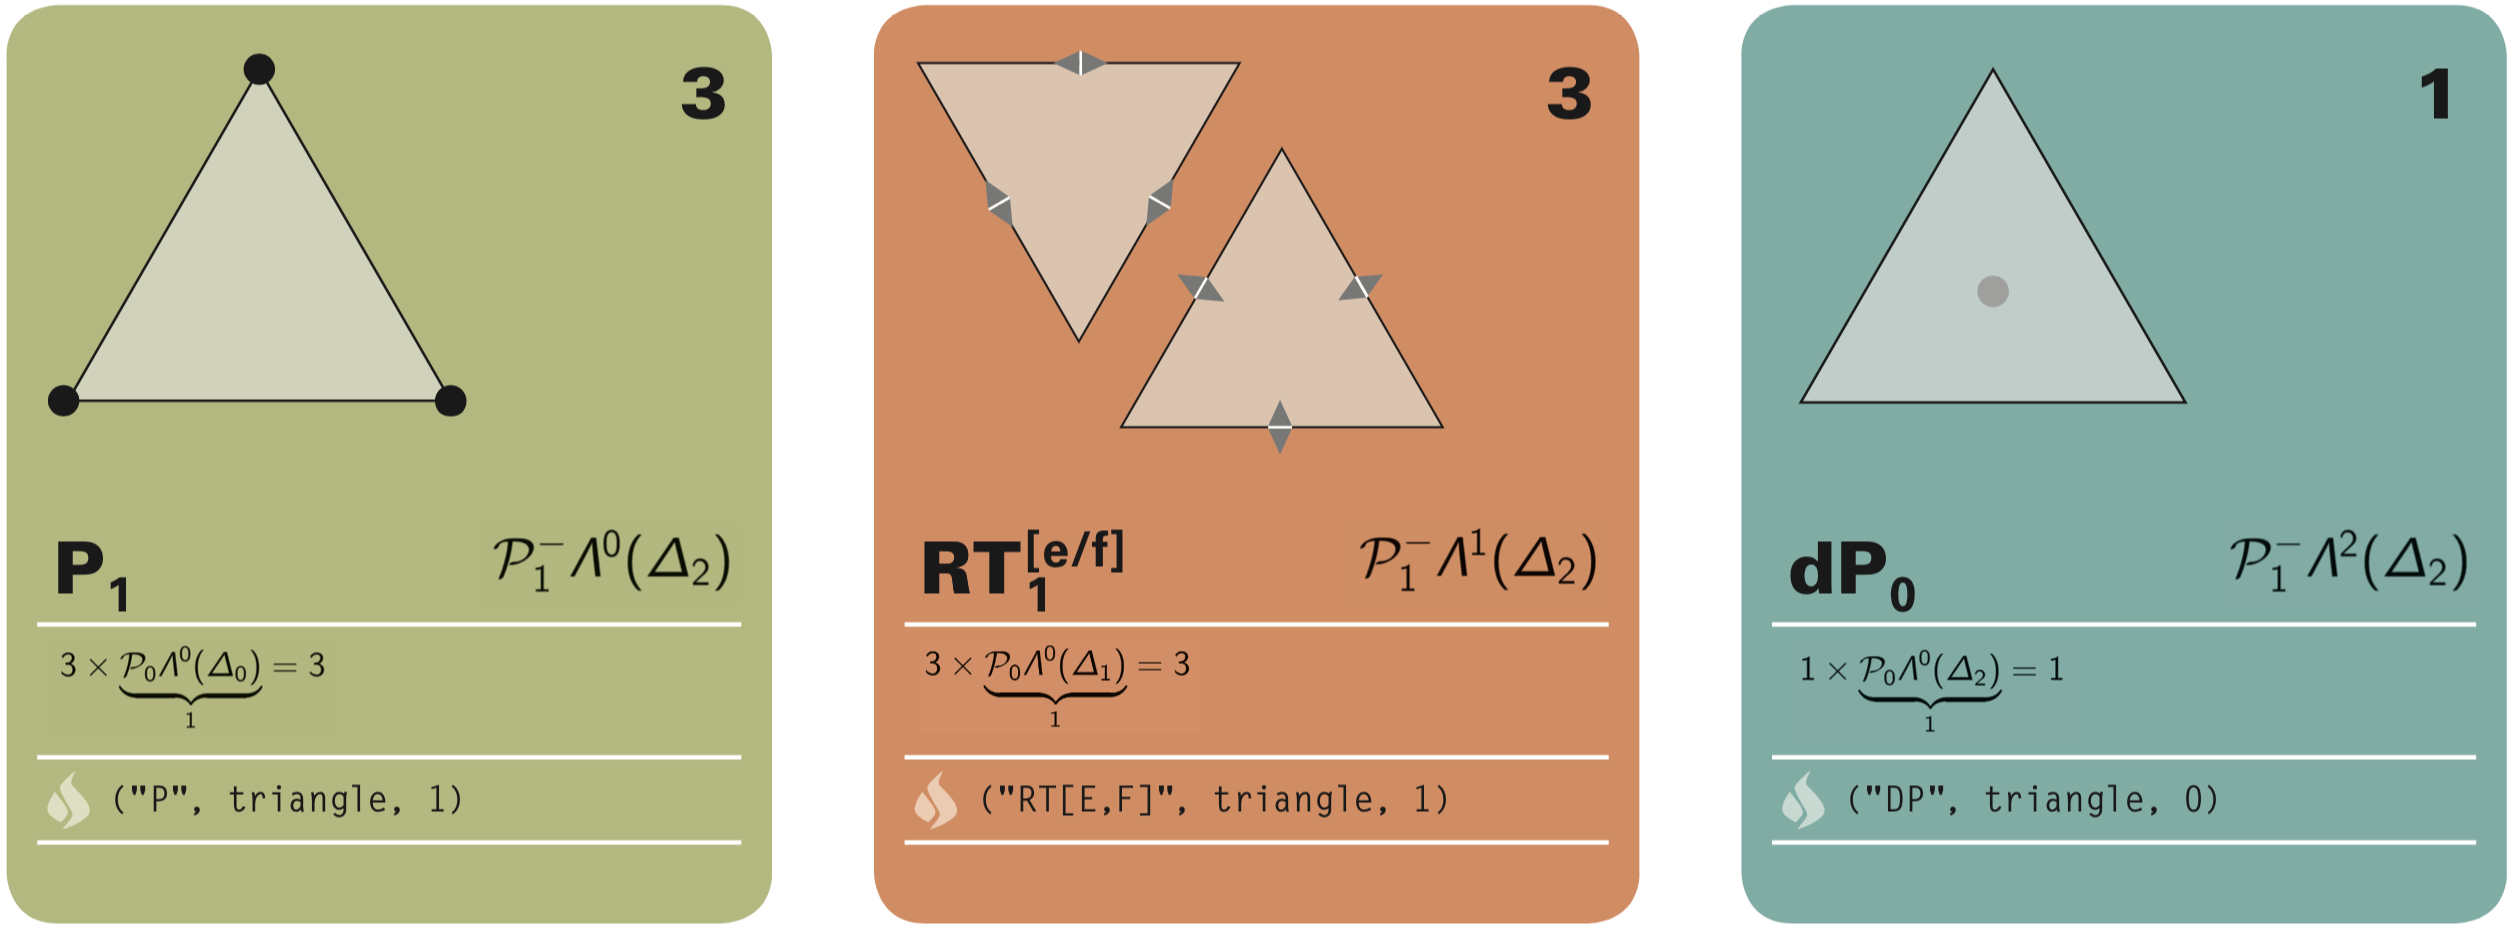
\includegraphics[width=0.5\textwidth]{rt-2d}
    \end{center}
    \vspace*{-\baselineskip}
    {\hfill \url{femtable.org}}
  \end{block}
  \pause
  \begin{columns}
    \begin{column}{0.7\textwidth}
      \begin{itemize}
      \item Exact sequence: $\ker(\div) = \range(\grad^\perp)$
      \item Need patches containing support of the $P_k$ basis
        functions $\Rightarrow$ star around vertices
      \end{itemize}
    \end{column}
    \begin{column}{0.3\textwidth}
      \begin{tikzpicture}[scale=2,
        on each segment/.style={
          decorate,
          decoration={
            show path construction,
            moveto code={},
            lineto code={
              \path [#1]
              (\tikzinputsegmentfirst) -- (\tikzinputsegmentlast);
            }}},
        dof/.style={postaction={decorate, decoration={markings,
              mark=at position 0.5 with {
                \node[transform shape,shape=diamond,fill,draw, inner
                sep=0pt, minimum height=5pt, minimum width=2.5pt] {};
              }}}}]
        \foreach \i/\k in {0/0, 0.5/1, 1/2} {
          \foreach \j/\l in {0/0, 0.5/1, 1/2} {
            \coordinate (v\k\l) at (\i, \j);
          }
        }

        \draw[thick, black, line join=miter, postaction={on each segment={dof}}] (v00)
        -- (v10) -- (v20) -- (v21) -- (v22) -- (v12) -- (v02) -- (v01) -- (v00);
        \draw[dof, thick, black, line join=cap] (v01) -- (v11);
        \draw[dof, thick, black, line join=cap] (v11) -- (v21);
        \draw[dof, thick, black, line join=cap] (v10) -- (v11);
        \draw[dof, thick, black, line join=cap] (v11) -- (v12);
        \draw[dof, thick, black, line join=cap] (v01) -- (v10);
        \draw[dof, thick, black, line join=cap] (v02) -- (v11);
        \draw[dof, thick, black, line join=cap] (v11) -- (v20);
        \draw[dof, thick, black, line join=cap] (v12) -- (v21);
        \coordinate (i10) at ($(v10) + (90:0.05)$);
        \coordinate (i20) at ($(v20) + (135:0.07071)$);
        \coordinate (i21) at ($(v21) + (180:0.05)$);
        \coordinate (i12) at ($(v12) + (270:0.05)$);
        \coordinate (i02) at ($(v02) + (315:0.07071)$);
        \coordinate (i01) at ($(v01) + (0:0.05)$);
        \path[fill=purple, opacity=0.5] \convexpath{i01,i02,i12,i21,i20,i10}{0.5pt};
      \end{tikzpicture}
    \end{column}
  \end{columns}
\end{frame}

\begin{frame}[fragile, t]
  \frametitle{{$H(\div)$ multigrid in 2D {\small \parencite{Arnold:1997}}}}
  \vspace*{-1.5\baselineskip}
  \begin{equation*}
    \text{Find $u \in V \subset H(\div)$ s.t.}\quad (u, v)_{L^2} + \gamma (\div u, \div v)_{L^2} = (f, v)_{L^2} \quad \forall v \in V.
  \end{equation*}
  \vspace{-\baselineskip}
  \begin{columns}
    \begin{column}{0.7\textwidth}
      {\scriptsize
\begin{verbatim}
    -ksp_type cg
    -pc_type mg
    -mg_levels_
       -pc_type python
       -pc_python_type firedrake.PatchPC
       -patch_
          -pc_patch_construct_dim 0
          -pc_patch_construct_type star
\end{verbatim}
}
    \end{column}
    \begin{column}{0.3\textwidth}
      \begin{center}
      \begin{tikzpicture}[scale=2,
        on each segment/.style={
          decorate,
          decoration={
            show path construction,
            moveto code={},
            lineto code={
              \path [#1]
              (\tikzinputsegmentfirst) -- (\tikzinputsegmentlast);
            }}},
        dof/.style={postaction={decorate, decoration={markings,
              mark=at position 0.5 with {
                \node[transform shape,shape=diamond,fill,draw, inner
                sep=0pt, minimum height=5pt, minimum width=2.5pt] {};
              }}}}]
        \foreach \i/\k in {0/0, 0.5/1, 1/2} {
          \foreach \j/\l in {0/0, 0.5/1, 1/2} {
            \coordinate (v\k\l) at (\i, \j);
          }
        }

        \draw[thick, black, line join=miter, postaction={on each segment={dof}}] (v00)
        -- (v10) -- (v20) -- (v21) -- (v22) -- (v12) -- (v02) -- (v01)
        -- (v00);
        \draw[dof, thick, black, line join=cap] (v01) -- (v11);
        \draw[dof, thick, black, line join=cap] (v11) -- (v21);
        \draw[dof, thick, black, line join=cap] (v10) -- (v11);
        \draw[dof, thick, black, line join=cap] (v11) -- (v12);
        \draw[dof, thick, black, line join=cap] (v01) -- (v10);
        \draw[dof, thick, black, line join=cap] (v02) -- (v11);
        \draw[dof, thick, black, line join=cap] (v11) -- (v20);
        \draw[dof, thick, black, line join=cap] (v12) -- (v21);
        \coordinate (i10) at ($(v10) + (90:0.05)$);
        \coordinate (i20) at ($(v20) + (135:0.07071)$);
        \coordinate (i21) at ($(v21) + (180:0.05)$);
        \coordinate (i12) at ($(v12) + (270:0.05)$);
        \coordinate (i02) at ($(v02) + (315:0.07071)$);
        \coordinate (i01) at ($(v01) + (0:0.05)$);
        \path[fill=purple, opacity=0.5]
        \convexpath{i01,i02,i12,i21,i20,i10}{0.5pt};
      \end{tikzpicture}
      \end{center}
    \end{column}
  \end{columns}    

  \begin{center}
    \begin{table}
      \begin{tabular}{l|cccccc}
        Smoother \textbackslash~ $\gamma$ & $0$ & $10^{-1}$ & $10^{0}$ & $10^{1}$ & $10^{2}$ & $10^{3}$ \\
        \midrule
        Point-Jacobi ($k=1$)  & 11 & 27 &  49 &68 &  86 & 103  \\
        Point-Jacobi  ($k=2$) & 10 & 45 &  71 & 93 & 113 & 134 \\
        \midrule
        Block-Jacobi  ($k=1$) &  6 & 11 &  12 & 12  &  12 & 12 \\
        Block-Jacobi  ($k=2$) &  7 & 8  &   8 & 8   &   8 & 8 
      \end{tabular}
      \caption{Iteration counts for multigrid preconditioned CG using
        $\text{RT}_k$ elements.}
    \end{table}
  \end{center}
\end{frame}

\begin{frame}[fragile,t]
  \frametitle{$H(\div)$ and $H(\curl)$ multigrid in 3D
    {\small \parencite{Arnold:2000}}}
  \vspace{-1.5\baselineskip}
  \begin{equation*}
    \text{Find $u \in V \subset H(\curl)$ s.t.}\quad (u, v)_{L^2} + \gamma (\curl u, \curl v)_{L^2} = (f, v)_{L^2} \quad \forall v \in V.
  \end{equation*}
  \vspace*{-\baselineskip}
  \begin{block}{$L^2$ de Rham complex}
    \begin{equation*}
      H^1 \xrightarrow{\grad} H(\curl) \xrightarrow{\curl} H(\div) \xrightarrow{\div} L^2
    \end{equation*}
    \vspace*{-2\baselineskip}
    \pause
    \begin{center}
      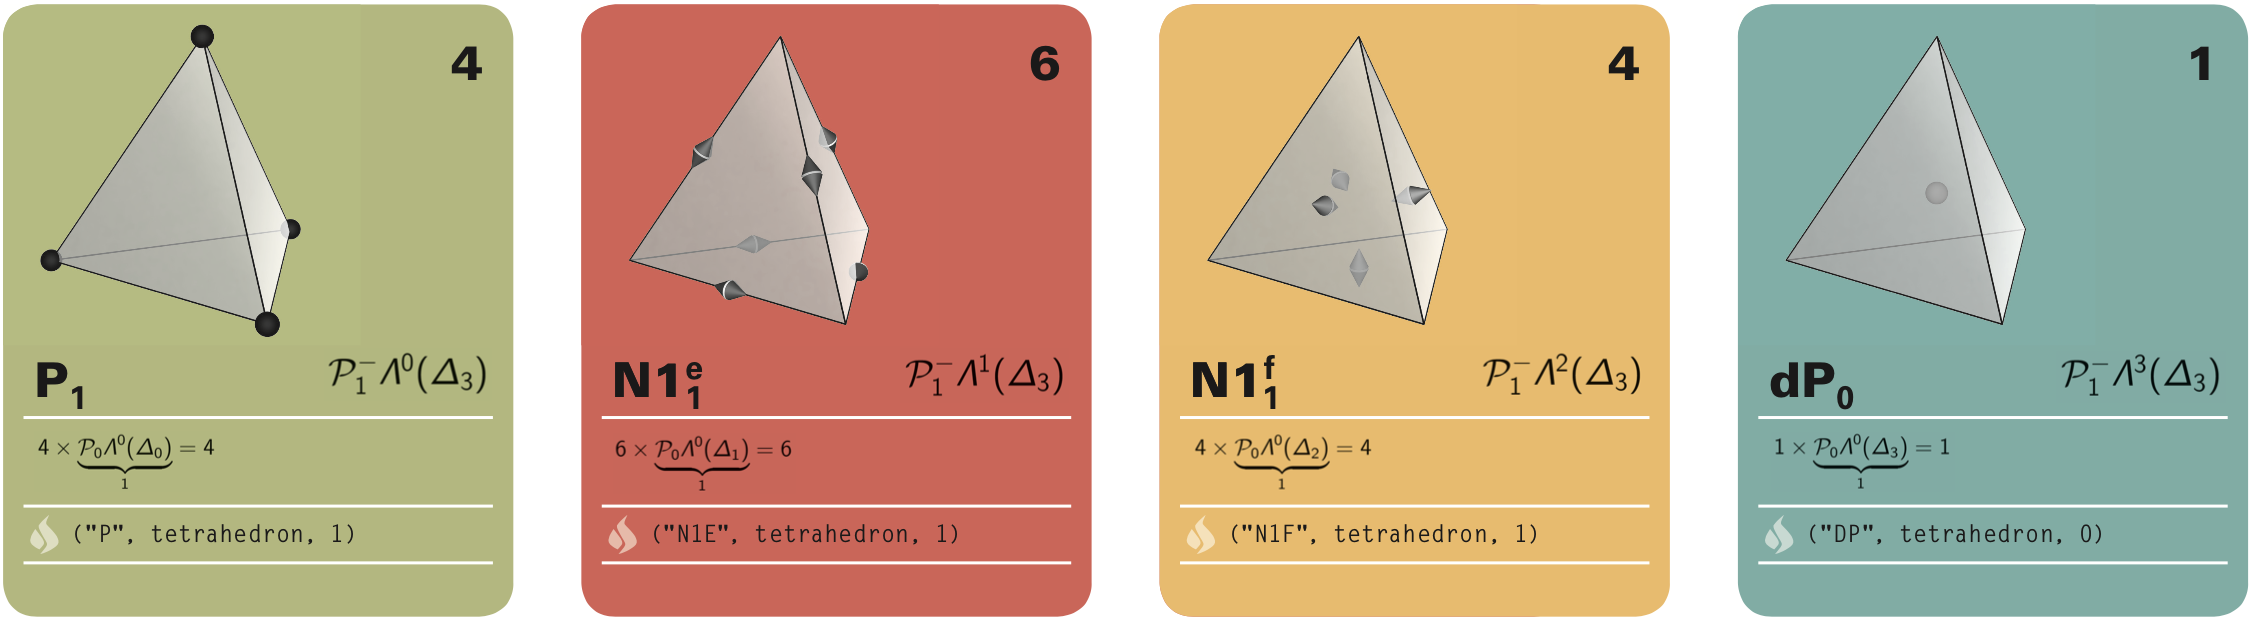
\includegraphics[width=0.5\textwidth]{rt-3d}
    \end{center}
    \vspace*{-\baselineskip}
    {\hfill \url{femtable.org}}
  \end{block}
  \begin{columns}
    \begin{column}{0.5\textwidth}
      \begin{itemize}
      \item Exact sequence: $\ker(\curl) = \range(\grad)$, $\ker(\div)
        = \range(\curl)$
      \item $H(\curl)$: star around vertices
      \item $H(\div)$: star around edges
      \end{itemize}
    \end{column}
    \begin{column}{0.5\textwidth}
      \begin{center}
      \begin{tikzpicture}[scale=2,
        on each segment/.style={
          decorate,
          decoration={
            show path construction,
            moveto code={},
            lineto code={
              \path [#1]
              (\tikzinputsegmentfirst) -- (\tikzinputsegmentlast);
            }}},
        nedof/.style={postaction={decorate, decoration={markings,
              mark=at position 0.5 with {
                \node[transform shape,shape=diamond,fill,draw, inner
                sep=0pt, minimum height=2.5pt, minimum width=5pt] {};
              }}}},
        rtdof/.style={postaction={decorate, decoration={markings,
              mark=at position 0.5 with {
                \node[transform shape,shape=diamond,fill,draw, inner
                sep=0pt, minimum height=5pt, minimum width=2.55pt] {};
              }}}}]
        \foreach \i/\k in {0/0, 0.5/1, 1/2} {
          \foreach \j/\l in {0/0, 0.5/1, 1/2} {
            \coordinate (v\k\l) at (\i, \j);
          }
        }

        \draw[thick, black, line join=miter, postaction={on each segment={nedof}}] (v00)
        -- (v10) -- (v20) -- (v21) -- (v22) -- (v12) -- (v02) -- (v01)
        -- (v00);
        \draw[nedof, thick, black, line join=cap] (v01) -- (v11);
        \draw[nedof, thick, black, line join=cap] (v11) -- (v21);
        \draw[nedof, thick, black, line join=cap] (v10) -- (v11);
        \draw[nedof, thick, black, line join=cap] (v11) -- (v12);
        \draw[nedof, thick, black, line join=cap] (v01) -- (v10);
        \draw[nedof, thick, black, line join=cap] (v02) -- (v11);
        \draw[nedof, thick, black, line join=cap] (v11) -- (v20);
        \draw[nedof, thick, black, line join=cap] (v12) -- (v21);
        \coordinate (i10) at ($(v10) + (90:0.05)$);
        \coordinate (i20) at ($(v20) + (135:0.07071)$);
        \coordinate (i21) at ($(v21) + (180:0.05)$);
        \coordinate (i12) at ($(v12) + (270:0.05)$);
        \coordinate (i02) at ($(v02) + (315:0.07071)$);
        \coordinate (i01) at ($(v01) + (0:0.05)$);
        \path[fill=purple, opacity=0.5]
        \convexpath{i01,i02,i12,i21,i20,i10}{0.5pt};

        \begin{scope}[shift={(1.5, 0)}]
          \foreach \i/\k in {0/0, 0.5/1, 1/2} {
            \foreach \j/\l in {0/0, 0.5/1, 1/2} {
              \coordinate (v\k\l) at (\i, \j);
            }
          }
          \draw[thick, black, line join=miter, postaction={on each segment={rtdof}}] (v00)
          -- (v10) -- (v20) -- (v21) -- (v22) -- (v12) -- (v02) -- (v01)
          -- (v00);
          \draw[rtdof, thick, black, line join=cap] (v01) -- (v11);
          \draw[rtdof, thick, black, line join=cap] (v11) -- (v21);
          \draw[rtdof, thick, black, line join=cap] (v10) -- (v11);
          \draw[rtdof, thick, black, line join=cap] (v11) -- (v12);
          \draw[rtdof, thick, black, line join=cap] (v01) -- (v10);
          \draw[rtdof, thick, black, line join=cap] (v02) -- (v11);
          \draw[rtdof, thick, black, line join=cap] (v11) -- (v20);
          \draw[rtdof, thick, black, line join=cap] (v12) -- (v21);


          \coordinate (e00) at ($(v00) + (45:0.07071)$);
          \coordinate (e10) at ($(v10) + (135:0.07071)$);
          \coordinate (e11) at ($(v11) + (225:0.07071)$);
          \coordinate (e01) at ($(v01) + (315:0.07071)$);

          \path[fill=purple, opacity=0.5]
          \convexpath{e00,e01,e11,e10}{0pt};

          \coordinate (o11) at ($(v11) + (90:0.03535)$);
          \coordinate (o21) at ($(v21) + (157.5:0.1)$);
          \coordinate (o12) at ($(v12) + (270:0.03535)$);
          \coordinate (o02) at ($(v02) + (337.5:0.1)$);

          \path[fill=purple, opacity=0.5]
          \convexpath{o11,o02,o12,o21}{0pt};
        \end{scope}
      \end{tikzpicture}
      \end{center}
    \end{column}
  \end{columns}
\end{frame}

\begin{frame}[fragile,t]
  \frametitle{$H(\curl)$ multigrid in 3D {\small \parencite{Arnold:2000}}}
  \vspace{-1.5\baselineskip}
  \begin{equation*}
    \text{Find $u \in V \subset H(\curl)$ s.t.}\quad (u, v)_{L^2} + \gamma (\curl u, \curl v)_{L^2} = (f, v)_{L^2} \quad \forall v \in V.
  \end{equation*}
  \vspace*{-\baselineskip}
  \begin{columns}
    \begin{column}{0.7\textwidth}
      {\scriptsize
\begin{verbatim}
    -ksp_type cg
    -pc_type mg
    -mg_levels_
       -pc_type python
       -pc_python_type firedrake.PatchPC
       -patch_
          -pc_patch_construct_dim 0
          -pc_patch_construct_type star
\end{verbatim}
      }
    \end{column}
    \begin{column}{0.3\textwidth}
      \begin{center}
        \begin{tikzpicture}[scale=2,
          on each segment/.style={
            decorate,
            decoration={
              show path construction,
              moveto code={},
              lineto code={
                \path [#1]
                (\tikzinputsegmentfirst) -- (\tikzinputsegmentlast);
              }}},
          dof/.style={postaction={decorate, decoration={markings,
                mark=at position 0.5 with {
                  \node[transform shape,shape=diamond,fill,draw, inner
                  sep=0pt, minimum height=2.5pt, minimum width=5pt] {};
                }}}}]
          \foreach \i/\k in {0/0, 0.5/1, 1/2} {
            \foreach \j/\l in {0/0, 0.5/1, 1/2} {
              \coordinate (v\k\l) at (\i, \j);
            }
          }

          \draw[thick, black, line join=miter, postaction={on each segment={dof}}] (v00)
          -- (v10) -- (v20) -- (v21) -- (v22) -- (v12) -- (v02) -- (v01)
          -- (v00);
          \draw[dof, thick, black, line join=cap] (v01) -- (v11);
          \draw[dof, thick, black, line join=cap] (v11) -- (v21);
          \draw[dof, thick, black, line join=cap] (v10) -- (v11);
          \draw[dof, thick, black, line join=cap] (v11) -- (v12);
          \draw[dof, thick, black, line join=cap] (v01) -- (v10);
          \draw[dof, thick, black, line join=cap] (v02) -- (v11);
          \draw[dof, thick, black, line join=cap] (v11) -- (v20);
          \draw[dof, thick, black, line join=cap] (v12) -- (v21);
          \coordinate (i10) at ($(v10) + (90:0.05)$);
          \coordinate (i20) at ($(v20) + (135:0.07071)$);
          \coordinate (i21) at ($(v21) + (180:0.05)$);
          \coordinate (i12) at ($(v12) + (270:0.05)$);
          \coordinate (i02) at ($(v02) + (315:0.07071)$);
          \coordinate (i01) at ($(v01) + (0:0.05)$);
          \path[fill=purple, opacity=0.5]
          \convexpath{i01,i02,i12,i21,i20,i10}{0.5pt};
        \end{tikzpicture}
      \end{center}
    \end{column}
  \end{columns}    

  \begin{center}
    \begin{table}
      \begin{tabular}{l|cccccc}
        % Hcurl
        Smoother \textbackslash{} $\gamma$ & $0$ & $10^{-1}$ & $10^{0}$ & $10^{1}$ & $10^{2}$ & $10^{3}$ \\
        \midrule
        Point-Jacobi ($k=1$)  & 10 & 48  &  85 & 120 & 150 & 180 \\
        Point-Jacobi  ($k=2$) & 22 & 115 & 211 & 293 & 370 & 446 \\
        \midrule
        Block-Jacobi  ($k=1$) &  9 & 16  &  18 & 18  &  18 & 18  \\
        Block-Jacobi  ($k=2$) &  9 & 12  &  12 & 12  &  12 & 12 
      \end{tabular}
      \caption{Iteration counts for multigrid preconditioned CG using Nedelec edge-elements of the first kind.}
    \end{table}
  \end{center}
\end{frame}

\begin{frame}[fragile,t]
  \frametitle{$H(\div)$ multigrid in 3D {\small \parencite{Arnold:2000}}}
  \vspace{-1.5\baselineskip}
  \begin{equation*}
    \text{Find $u \in V \subset H(\div)$ s.t.}\quad (u, v)_{L^2} + \gamma (\div u, \div v)_{L^2} = (f, v)_{L^2} \quad \forall v \in V.
  \end{equation*}
  \vspace*{-\baselineskip}
  \begin{columns}
    \begin{column}{0.7\textwidth}
      {\scriptsize
\begin{verbatim}
    -ksp_type cg
    -pc_type mg
    -mg_levels_
       -pc_type python
       -pc_python_type firedrake.PatchPC
       -patch_
          -pc_patch_construct_dim 1
          -pc_patch_construct_type star
\end{verbatim}
      }
    \end{column}
    \begin{column}{0.3\textwidth}
      \begin{center}
        \begin{tikzpicture}[scale=2,
          on each segment/.style={
            decorate,
            decoration={
              show path construction,
              moveto code={},
              lineto code={
                \path [#1]
                (\tikzinputsegmentfirst) -- (\tikzinputsegmentlast);
              }}},
          dof/.style={postaction={decorate, decoration={markings,
                mark=at position 0.5 with {
                  \node[transform shape,shape=diamond,fill,draw, inner
                  sep=0pt, minimum height=5pt, minimum width=2.5pt] {};
                }}}}]
          \foreach \i/\k in {0/0, 0.5/1, 1/2} {
            \foreach \j/\l in {0/0, 0.5/1, 1/2} {
              \coordinate (v\k\l) at (\i, \j);
            }
          }

          \draw[thick, black, line join=miter, postaction={on each segment={dof}}] (v00)
          -- (v10) -- (v20) -- (v21) -- (v22) -- (v12) -- (v02) -- (v01)
          -- (v00);
          \draw[dof, thick, black, line join=cap] (v01) -- (v11);
          \draw[dof, thick, black, line join=cap] (v11) -- (v21);
          \draw[dof, thick, black, line join=cap] (v10) -- (v11);
          \draw[dof, thick, black, line join=cap] (v11) -- (v12);
          \draw[dof, thick, black, line join=cap] (v01) -- (v10);
          \draw[dof, thick, black, line join=cap] (v02) -- (v11);
          \draw[dof, thick, black, line join=cap] (v11) -- (v20);
          \draw[dof, thick, black, line join=cap] (v12) -- (v21);


          \coordinate (e00) at ($(v00) + (45:0.07071)$);
          \coordinate (e10) at ($(v10) + (135:0.07071)$);
          \coordinate (e11) at ($(v11) + (225:0.07071)$);
          \coordinate (e01) at ($(v01) + (315:0.07071)$);

          \path[fill=purple, opacity=0.5]
          \convexpath{e00,e01,e11,e10}{0pt};

          \coordinate (o11) at ($(v11) + (90:0.03535)$);
          \coordinate (o21) at ($(v21) + (157.5:0.1)$);
          \coordinate (o12) at ($(v12) + (270:0.03535)$);
          \coordinate (o02) at ($(v02) + (337.5:0.1)$);

          \path[fill=purple, opacity=0.5]
          \convexpath{o11,o02,o12,o21}{0pt};
        \end{tikzpicture}
      \end{center}
    \end{column}
  \end{columns}    
  \begin{center}
    \begin{table}
      \begin{tabular}{l|cccccc}
        % Hdiv
        Smoother \textbackslash{} $\gamma$ & $0$ & $10^{-1}$ & $10^{0}$ & $10^{1}$ & $10^{2}$ & $10^{3}$ \\
        \midrule
        Point-Jacobi ($k=1$)  & 11 & 63  & 109 & 146 & 180 & 221 \\
        Point-Jacobi  ($k=2$) & 26 & 180 & 366 & 531 & 687 & 844 \\
        \midrule
        Block-Jacobi  ($k=1$) & 12 & 30  &  36 & 36  &  37 & 37  \\
        Block-Jacobi  ($k=2$) & 11 & 17  &  17 & 17  &  17 & 17
      \end{tabular}
      \caption{Iteration counts for multigrid preconditioned CG using Nedelec face-elements of the first kind.}
    \end{table}
    \end{center}
\end{frame}

\begin{frame}[fragile,t]
  \frametitle{Nearly incompressible elasticity}
  \vspace*{-1.5\baselineskip}
  \begin{equation*}
    \text{Find $u \in V \subset H^1$ s.t.} \quad (\grad u, \grad v) + \gamma (\div u, \div v) = (f, v) \quad \forall v \in V.
  \end{equation*}
  \vspace*{-\baselineskip}
  \begin{block}{2D Stokes complex}
    \begin{equation*}
      H^2 \xrightarrow{\grad^\perp} H^1 \xrightarrow{\div} L^2
    \end{equation*}
    \vspace*{-\baselineskip}
    \begin{center}
      \includestandalone[width=0.5\textwidth]{./../pictures/HCT-complex}
    \end{center}
    \begin{itemize}
    \item Decomposition must capture $\ker \div = \range \grad^\perp$.
    \item Support of HCT element is on ``macro'' mesh $\Rightarrow$ \texttt{MacroStar}
    \end{itemize}
  \end{block}
\end{frame}
\begin{frame}[fragile]
  \frametitle{\texttt{MacroStar}}
  \begin{onlyenv}<1-3>
    \begin{center}
      \begin{tikzpicture}[scale=2,
        bcdof/.style={postaction={decorate,decoration={markings,
              mark=at position 0.5 with {\draw[solid, fill, black!60] circle
                (0.06);}}}},
        dof/.style={postaction={decorate,decoration={markings,
              mark=at position 0.5 with {\draw[solid, fill, black] circle (0.06);}}}
        }]

        \foreach \i in {0, 1, 2, 3} {
          \coordinate (0-\i) at ($(\i*1.5, 0)$);
          \coordinate (1-\i) at ($(0-\i) + (60:1.5)$);
          \coordinate (2-\i) at ($(1-\i) + (120:1.5)$);
        }
        \foreach \i/\j in {0/1, 1/2, 2/3} {
          \foreach \k in {0, 2} {
            \draw[line join=miter, very thick] (\k-\i) -- (\k-\j);
          }
          \draw[line join=miter, very thick] (0-\i) -- (1-\i);
          \draw[line join=miter, very thick] (1-\i) -- (2-\i);
          \draw[line join=miter, very thick] (0-\j) -- (1-\i);
          \draw[line join=miter, very thick] (1-\i) -- (2-\j);
        }

        \foreach \i/\j in {0/1, 1/2} {
          \draw[line join=miter, very thick] (1-\i) -- (1-\j);
        }
        \foreach \i/\j in {0/1, 1/2, 2/3} {
          \coordinate (bc-0-\i-\j) at (barycentric cs:0-\i=1,0-\j=1,1-\i=1);
          \draw[line join=miter, dotted, thick] (0-\i) -- (bc-0-\i-\j);
          \draw[line join=miter, dotted, thick] (1-\i) -- (bc-0-\i-\j);
          \draw[line join=miter, dotted, thick] (0-\j) -- (bc-0-\i-\j);

          \coordinate (bc-2-\i-\j) at (barycentric cs:1-\i=1,2-\i=1,2-\j=1);
          \draw[line join=miter, dotted, thick] (1-\i) -- (bc-2-\i-\j);
          \draw[line join=miter, dotted, thick] (2-\i) -- (bc-2-\i-\j);
          \draw[line join=miter, dotted, thick] (2-\j) -- (bc-2-\i-\j);
        }
        \foreach \i/\j in {0/1, 1/2} { 
          \coordinate (bc-1-\i-\j)  at (barycentric cs:1-\i=1,0-\j=1,1-\j=1);
          \draw[line join=miter, dotted, thick] (1-\i) -- (bc-1-\i-\j);
          \draw[line join=miter, dotted, thick] (0-\j) -- (bc-1-\i-\j);
          \draw[line join=miter, dotted, thick] (1-\j) -- (bc-1-\i-\j);

          \coordinate (bc-3-\i-\j)  at (barycentric cs:1-\i=1,1-\j=1,2-\j=1);
          \draw[line join=miter, dotted, thick] (1-\i) -- (bc-3-\i-\j);
          \draw[line join=miter, dotted, thick] (1-\j) -- (bc-3-\i-\j);
          \draw[line join=miter, dotted, thick] (2-\j) -- (bc-3-\i-\j);
        }

        \pause

        \path[fill=purple, opacity=0.5] ([shift={(0:4pt)}]1-0) --
        ([shift={(60:4pt)}]0-1) --
        ([shift={(120:4pt)}]0-2) --
        ([shift={(180:4pt)}]1-2) --
        ([shift={(240:4pt)}]2-2) --
        ([shift={(300:4pt)}]2-1) --
        cycle;

        \pause

        \foreach \i in {0, 1, 2, 3} {
          \foreach \j in {0, 2} {
            \draw[fill, black] (\j-\i) circle (0.05);
          }
        }
        \foreach \i in {0, 1, 2} {
          \draw[fill] (1-\i) circle (0.05);
        }
        \foreach \i/\j in {0/1, 1/2, 2/3} {
          \foreach \k in {0, 2} {
            \draw[fill] (bc-\k-\i-\j) circle (0.05);
          }
        }
        \foreach \i/\j in {0/1, 1/2} { 
          \foreach \k in {1, 3} {
            \draw[fill] (bc-\k-\i-\j) circle (0.05);
          }
        }

        \foreach \i/\j in {0/1, 1/2, 2/3} {
          \draw[fill] (barycentric cs:0-\i=1,0-\j=1) circle (0.05);
          \draw[fill] (barycentric cs:2-\i=1,2-\j=1) circle (0.05);
          \draw[fill] (barycentric cs:0-\i=1,1-\i=1) circle (0.05);
          \draw[fill] (barycentric cs:0-\j=1,1-\i=1) circle (0.05);
          \draw[fill] (barycentric cs:1-\i=1,2-\i=1) circle (0.05);
          \draw[fill] (barycentric cs:1-\i=1,2-\j=1) circle (0.05);
        }
        \draw[fill] (barycentric cs:1-0=1,1-1=1) circle (0.05);
        \draw[fill] (barycentric cs:1-1=1,1-2=1) circle (0.05);

        \foreach \i in {0-0, 0-1, 1-0} {
          \draw[fill] (barycentric cs:\i=1,bc-0-0-1=1) circle (0.05);
        }
        \foreach \i in {0-1, 0-2, 1-1} {
          \draw[fill] (barycentric cs:\i=1,bc-0-1-2=1) circle (0.05);
        }
        \foreach \i in {0-2, 0-3, 1-2} {
          \draw[fill] (barycentric cs:\i=1,bc-0-2-3=1) circle (0.05);
        }
        \foreach \i in {2-0, 2-1, 1-0} {
          \draw[fill] (barycentric cs:\i=1,bc-2-0-1=1) circle (0.05);
        }
        \foreach \i in {2-1, 2-2, 1-1} {
          \draw[fill] (barycentric cs:\i=1,bc-2-1-2=1) circle (0.05);
        }
        \foreach \i in {2-2, 2-3, 1-2} {
          \draw[fill] (barycentric cs:\i=1,bc-2-2-3=1) circle (0.05);
        }
        \foreach \i in {0-1, 1-0, 1-1} {
          \draw[fill] (barycentric cs:\i=1,bc-1-0-1=1) circle (0.05);
        }
        \foreach \i in {0-2, 1-1, 1-2} {
          \draw[fill] (barycentric cs:\i=1,bc-1-1-2=1) circle (0.05);
        }
        \foreach \i in {1-0, 2-1, 1-1} {
          \draw[fill] (barycentric cs:\i=1,bc-3-0-1=1) circle (0.05);
        }
        \foreach \i in {1-1, 2-2, 1-2} {
          \draw[fill] (barycentric cs:\i=1,bc-3-1-2=1) circle (0.05);
        }
      \end{tikzpicture}
    \end{center}
  \end{onlyenv}
  \begin{onlyenv}<4->
    {\scriptsize
\begin{verbatim}
-ksp_type cg
-pc_type mg
-mg_levels_
  -pc_type python
  -pc_python_type firedrake.PatchPC
    -patch_
      -pc_patch_construct_dim 0
      -pc_patch_construct_type python
      -pc_patch_construct_python_type MacroStar
\end{verbatim}
    }
    Just need to write custom adjacency to construct patch around each vertex
    \begin{uncoverenv}<5->
\begin{minted}[fontsize=\scriptsize]{python}
class MacroStar(OrderedRelaxation):
    def callback(self, dm, vertex):
        if dm.getLabelValue("MacroVertices", vertex) != 1:
            return None
        s = list(self.star(dm, vertex))
        closures = list(chain(*(self.closure(dm, e) for e in s)))
        want = [v for v in closures if dm.getLabelValue("MacroVertices", v) != 1]
        star = list(chain(*(self.star(dm, v) for v in want)))
        return s + star
\end{minted}
    \end{uncoverenv}
  \end{onlyenv}
\end{frame}

\begin{frame}[fragile, t]
  \frametitle{Vanka for Stokes}
  Find $(u, p) \in V\times Q \subset (H^1)^d \times L^2$ s.t.
  \begin{equation*}
    (\grad u, \grad v) - (p, \div v) - (\div u, q) = (f, v) \quad \forall (v, q) \in V \times Q.
  \end{equation*}

  \begin{block}{Vanka patch}
    Solve simultaneously for $(u, p)$ on each pressure dof, gathering
    those velocity dofs that couple to the pressure dof.
    \vspace*{-0.5\baselineskip}
    \begin{itemize}
    \only<1-2>{\item \textbf{P2-P0: loop over cells, gather closure of
          star}}
    \only<3->{\item P2-P0: loop over cells, gather closure of star}
    \only<1-2>{\item P2-P1: loop over vertices, gather closure
      of star}
    \only<3->{\item \textbf{P2-P1: loop over vertices, gather closure of star}}
    \end{itemize}
    \nocite{Vanka:1986}
  \end{block}
  \vspace*{-1\baselineskip}
  \begin{overlayarea}{\textwidth}{0.52\textheight}
    \begin{onlyenv}<2>
      \begin{columns}[T]
        \begin{column}{0.5\textwidth}
          \begin{center}
            \begin{tikzpicture}[scale=2.5]
              \foreach \i/\k in {0/0, 0.5/1, 1/2} {
                \foreach \j/\l in {0/0, 0.5/1, 1/2} {
                  \coordinate (v\k\l) at (\i, \j);
                  \draw[fill] (v\k\l) circle (0.02);
                }
              }

              \draw[thick, black, line join=miter] (v00) -- (v10) -- (v20) -- (v21) -- (v22) -- (v12) -- (v02) -- (v01) -- cycle;
              \draw[thick, black, line join=miter] (v01) -- (v11) -- (v21);
              \draw[thick, black, line join=miter] (v10) -- (v11) -- (v12);
              \draw[thick, black, line join=miter] (v01) -- (v10);
              \draw[thick, black, line join=miter] (v02) -- (v11) -- (v20);
              \draw[thick, black, line join=miter] (v12) -- (v21);

              \foreach \i/\j in {0/1, 1/2} {
                \foreach \k in {0, 1, 2} {
                  \draw[fill] (barycentric cs:v\i\k=1,v\j\k=1) circle (0.02);
                  \draw[fill] (barycentric cs:v\k\i=1,v\k\j=1) circle (0.02);
                }
              }

              \draw[fill] (barycentric cs:v10=1,v01=1) circle (0.02);
              \draw[fill] (barycentric cs:v21=1,v12=1) circle (0.02);
              \draw[fill] (barycentric cs:v20=1,v11=1) circle (0.02);
              \draw[fill] (barycentric cs:v11=1,v02=1) circle (0.02);

              \node[shape=diamond,fill=red,red,draw, inner sep=0pt,
              minimum height=7pt, minimum width=7pt] at (barycentric cs:v00=1,v10=1,v01=1) {};

              \node[shape=diamond,fill=red,red,draw, inner sep=0pt,
              minimum height=7pt, minimum width=7pt] at (barycentric cs:v11=1,v10=1,v01=1) {};

              \node[shape=diamond,fill=red,red,draw, inner sep=0pt,
              minimum height=7pt, minimum width=7pt] at (barycentric cs:v11=1,v10=1,v20=1) {};

              \node[shape=diamond,fill=red,red,draw, inner sep=0pt,
              minimum height=7pt, minimum width=7pt] at (barycentric cs:v11=1,v21=1,v20=1) {};

              \node[shape=diamond,fill=red,red,draw, inner sep=0pt,
              minimum height=7pt, minimum width=7pt] at (barycentric cs:v01=1,v11=1,v02=1) {};

              \node[shape=diamond,fill=red,red,draw, inner sep=0pt,
              minimum height=7pt, minimum width=7pt] at (barycentric cs:v12=1,v11=1,v02=1) {};

              \node[shape=diamond,fill=red,red,draw, inner sep=0pt,
              minimum height=7pt, minimum width=7pt] at (barycentric cs:v12=1,v11=1,v21=1) {};

              \node[shape=diamond,fill=red,red,draw, inner sep=0pt,
              minimum height=7pt, minimum width=7pt] at (barycentric cs:v12=1,v22=1,v21=1) {};


              \coordinate (o11) at ($(v11) + (225:0.0866)$);
              \coordinate (o12) at ($(v12) + (112.5:0.1412)$);
              \coordinate (o21) at ($(v21) + (337.5:0.1412)$);

              \path[fill=purple, opacity=0.5] \convexpath{o11,o12,o21}{0.5pt};
              \phantom{\draw (-0.2,-0.2) -- (1.2, -0.2) -- (1.2, 1.2)
                -- (-0.2, 1.2) -- cycle;}
            \end{tikzpicture}
          \end{center}
        \end{column}
        \begin{column}{0.5\textwidth}
          {\scriptsize
\begin{verbatim}
-ksp_type gmres
-pc_type mg
-mg_levels_
   -pc_type python
   -pc_python_type firedrake.PatchPC
   -patch_
      -pc_patch_construct_codim 0
      -pc_patch_construct_type vanka
      -pc_patch_exclude_subspaces 1

\end{verbatim}
          }
        \end{column}
      \end{columns}
    \end{onlyenv}
    \begin{onlyenv}<3->
      \begin{columns}[T]
        \begin{column}{0.5\textwidth}
          \begin{center}
            \begin{tikzpicture}[scale=2.5]
              \foreach \i/\k in {0/0, 0.5/1, 1/2} {
                \foreach \j/\l in {0/0, 0.5/1, 1/2} {
                  \coordinate (v\k\l) at (\i, \j);
                }
              }
              \coordinate (o20) at ($(v20) + (315:0.1)$);
              \coordinate (o21) at ($(v21) + (0:0.0707)$);
              \coordinate (o12) at ($(v12) + (90:0.0707)$);
              \coordinate (o02) at ($(v02) + (135:0.1)$);
              \coordinate (o01) at ($(v01) + (180:0.0707)$);
              \coordinate (o10) at ($(v10) + (270:0.0707)$);

              \path[fill=purple, opacity=0.5]
              \convexpath{o10,o01,o02,o12,o21,o20}{0.5pt};

              \foreach \i in {10,20,21,12,02,01} {
                \node[shape=circle,draw,white,fill=white,inner
                sep=0pt, minimum size=20pt] at (v\i) {};
              }
              
              \foreach \i/\k in {0/0, 0.5/1, 1/2} {
                \foreach \j/\l in {0/0, 0.5/1, 1/2} {
                  \node[shape=diamond,draw,red, fill=red,inner
                  sep=0pt,
                  minimum height=7pt, minimum width=7pt] at (v\k\l) {};
                  \draw[fill] (v\k\l) circle (0.02);
                }
              }

              \draw[thick, black, line join=miter] (v00) -- (v10) -- (v20) -- (v21) -- (v22) -- (v12) -- (v02) -- (v01) -- cycle;
              \draw[thick, black, line join=miter] (v01) -- (v11) -- (v21);
              \draw[thick, black, line join=miter] (v10) -- (v11) -- (v12);
              \draw[thick, black, line join=miter] (v01) -- (v10);
              \draw[thick, black, line join=miter] (v02) -- (v11) -- (v20);
              \draw[thick, black, line join=miter] (v12) -- (v21);

              \foreach \i/\j in {0/1, 1/2} {
                \foreach \k in {0, 1, 2} {
                  \draw[fill] (barycentric cs:v\i\k=1,v\j\k=1) circle (0.02);
                  \draw[fill] (barycentric cs:v\k\i=1,v\k\j=1) circle (0.02);
                }
              }

              \draw[fill] (barycentric cs:v10=1,v01=1) circle (0.02);
              \draw[fill] (barycentric cs:v21=1,v12=1) circle (0.02);
              \draw[fill] (barycentric cs:v20=1,v11=1) circle (0.02);
              \draw[fill] (barycentric cs:v11=1,v02=1) circle (0.02);

              \phantom{\draw (-0.2,-0.2) -- (1.2, -0.2) -- (1.2, 1.2)
                -- (-0.2, 1.2) -- cycle;}
            \end{tikzpicture}
          \end{center}
        \end{column}
        \begin{column}{0.5\textwidth}
          {\scriptsize
\begin{verbatim}
-ksp_type gmres
-pc_type mg
-mg_levels_
   -pc_type python
   -pc_python_type firedrake.PatchPC
   -patch_
      -pc_patch_construct_dim 0
      -pc_patch_construct_type vanka
      -pc_patch_exclude_subspaces 1
      -pc_patch_vanka_dim 0
\end{verbatim}
          }
        \end{column}
      \end{columns}
    \end{onlyenv}
  \end{overlayarea}
\end{frame}

\begin{frame}
  \frametitle{Conclusions}
  \begin{itemize}
  \item \texttt{PCPATCH} provides simple and flexible interface for
    subspace correction methods
  \item Currently works with \texttt{DMPlex} + \texttt{PetscDS} and
    Firedrake
  \item Implements
    \begin{itemize}
    \item Additive and multiplicative smoothing
    \item Simultaneous smoothing of multiple fields: monolithic
      approaches
    \item Partition of unity (or not)
    \item Nonlinear relaxation (Firedrake only)
    \end{itemize}
  \end{itemize}

  \begin{center}
    Thanks!
  \end{center}
\end{frame}

\appendix
\begin{frame}
  \frametitle{References}
  \printbibliography[heading=none]
\end{frame}


\end{document}

